\chapter{상대론적 장으로서의 전기와 자기}

주어진 전자기장 속에서 대전 입자가 어떻게 운동하는지 살펴보았다. 문제의 나머지 절반은 아직 다루지 않았다. 장 자체, 즉 전기장과 자기장이 어떻게 변하는지, 전하와 전류가 어떻게 그 원천으로 작용하는지이다. 맥스웰 방정식이 이 질문들에 답한다. 하지만 방정식을 쓰기에 앞서, 전기장과 자기장의 상대론적 구조가 불가피해진 물리적 수수께끼를 되짚어 볼 만하다.

여기서는 의도적으로 형식론에서 한발 물러선다. 작용 원리는 다시 다루겠지만, 아직은 아니다. 먼저 다른 곳에서 시작하는 이유는 전기장과 자기장의 동역학을 작용으로부터 유도하기 전에, 두 장이 왜 하나의 대상의 일부여야 하는지 살펴보기 위해서다.

\section{아인슈타인 논문 첫 문단의 수수께끼}

벨기에를 방문했을 때 초기 솔베이 회의에 관한 이야기를 나누다가 아인슈타인의 1905년 논문 \emph{운동하는 물체의 전기역학에 대하여}로 화제가 옮겨 갔다. 논문의 첫 문단은 동기를 놀라울 만큼 간결하게 제시한다. 동일한 전자기 현상이 두 관성계에서 겉보기에는 서로 다른 설명을 받는다. 한 관찰자는 그 효과를 자기적인 것으로, 다른 관찰자는 전기적인 것으로 설명한다. 관측되는 운동은 서로 일치하므로, 두 설명이 서로 다른 두 가지 물리를 나타낼 수는 없다.

이제 이 논문을 이 강의에서 다룬 수준으로 이해할 수 있다. 모든 계산을 따라가지 않더라도, 답을 제시하기 전에 올바른 질문을 던지는 첫 문단은 읽어 볼 가치가 있다. 물리적 사건은 그대로인데 전기적 설명과 자기적 설명은 어떻게 달라질 수 있을까?

\subsection{전하와 자석, 그리고 두 가지 설명}

\(y\) 방향을 향하는 자기장을 두고, 전하가 \(x\)축을 따라 움직인다고 하자. 실험실 기준계에서는 전기장이 사라지므로 힘은 자기력이다:
\begin{equation}
\mathbf F=q\,\mathbf v\times\mathbf B.
\end{equation}
힘은 나머지 횡방향을 향한다. 강의에서 칠판에 빠르게 그린 축은 오른손 법칙의 부호를 하나하나 정하려는 것이 아니다. 중요한 점은 힘이 \(\mathbf v\)와 \(\mathbf B\) 모두에 수직이며, 전하의 부호를 바꾸면 힘의 방향도 반대가 된다는 것이다.

\begin{classroomqa}\audiencequestion{그림에서 힘은 위쪽을 향하나요, 아래쪽을 향하나요?}\lecturerresponse{전하의 부호에 따라 달라진다. 좌표축의 방향과 \(q\)의 부호가 정해지면 오른손 법칙으로 방향을 결정할 수 있다. 여기서 논의하는 데에는 횡방향 힘이 존재한다는 사실만 중요하다. \lecturetimestamp{00:07:13}}\end{classroomqa}

아인슈타인은 고립된 입자 대신 도선을 설명했다. 원자들은 대략 고정된 격자를 이루고, 이동 가능한 전하 운반자들은 그 안에서 움직인다. 20세기 초에는 도선에 흐르는 전류가 자유 대전 입자 하나의 궤적보다 관측하기도 훨씬 쉬웠다. 여기서는 이 구분이 본질적이지 않다. 자기장 속에서 움직이는 전하 운반자는 동일한 로런츠 힘을 받는다.

\begin{figure}[H]\centering
\includegraphics[width=\linewidth]{lecture_08_figure_01.png}\caption{아인슈타인의 전기역학 수수께끼를 다시 설명하는 데 쓰인 움직이는 전하, 횡방향 자기장, 자석의 배치.}\par\smallskip
\textit{강의 화면: 00:07:00.}\end{figure}

이번에는 도선이나 시험 전하는 고정해 두고 자석만 움직이자. 자기 배치가 변하면 기전력이 생기며, 국소적인 설명에서는 이를 전기장이라고 한다. 그 전기장은 정지해 있는 전하를 같은 횡방향으로 민다. 따라서 두 가지 설명은 다음과 같다.
\begin{align}
\text{moving charge, fixed magnet:}\quad&
q\,\mathbf v\times\mathbf B,
\\
\text{fixed charge, moving magnet:}\quad&
q\,\mathbf E'.
\end{align}
상대 운동은 동일하다. 그러므로 상대론은 한 기준계에서 순수하게 자기적인 장이 다른 기준계에서는 어떻게 전기 성분을 갖게 되는지 설명해야 한다.

전기와 자기는 서로 분리된 물질이 아니다. 하나의 상대론적 장이 기준계에 따라 전기적인 부분과 자기적인 부분으로 나뉘어 보이는 것이다. 아인슈타인은 아직 현대적인 장 텐서 표기법을 갖고 있지 않았고, 이 문단에서 필요한 기준계 변환을 로런츠 변환이라고 부르지도 않았다. 그렇지만 변환에 관한 질문은 이미 온전히 제기되어 있다.

\section{전자기장 텐서}

전기장과 자기장의 정보를 함께 담을 수 있는 대상은 반대칭 텐서다.
\begin{equation}
F_{\mu\nu}
=
\partial_\mu A_\nu-\partial_\nu A_\mu.
\label{eq:field-tensor-definition}
\end{equation}
그리스 첨자는 \(0,1,2,3\)의 값을 가지며, \(x^0=t\)이다. 라틴 첨자는 세 공간 방향의 값을 갖는다. 반대칭성
\begin{equation}
F_{\mu\nu}=-F_{\nu\mu},
\end{equation}
에 따라 대각 성분은 0이고 독립 성분은 여섯 개만 남는다. 이 여섯 성분은 정확히 \(\mathbf E\)의 세 성분과 \(\mathbf B\)의 세 성분이다.

대각 성분이 \begin{equation}
\eta_{\mu\nu}=\operatorname{diag}(-1,1,1,1),
\end{equation}인 대부분 양의 계량과 앞선 강의의 대전 입자 작용에서 이어받은 규약을 사용하여 다음과 같이 정의한다.
\begin{align}
E_m&=F_{0m}
=\partial_0A_m-\partial_mA_0,
\label{eq:e-from-a}
\\
B_i&=(\boldsymbol\nabla\times\mathbf A)_i.
\label{eq:b-from-a}
\end{align}
첫째 줄을 쓰는 과정에서 강의 중 공간 첨자 하나가 잘못 적혔다. 위에 쓴 식이 올바른 관계다. 자유 공간 첨자는 양변에서 일치해야 한다.

\begin{figure}[H]\centering
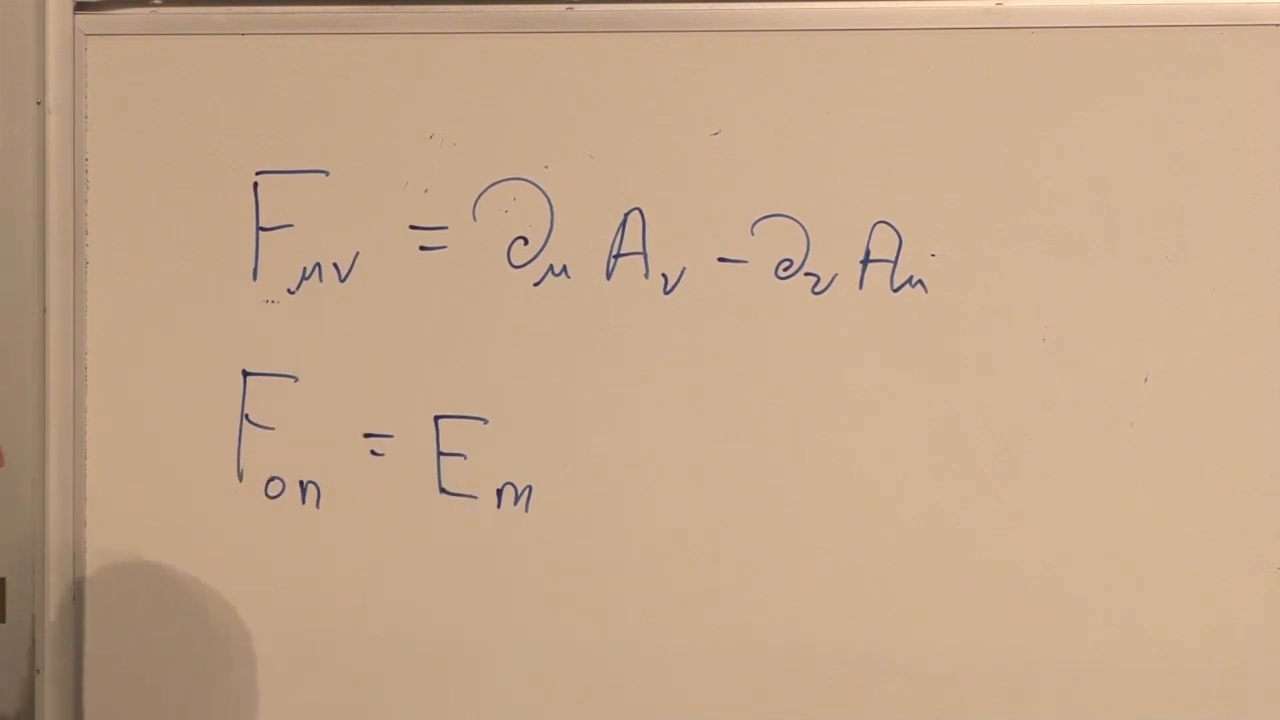
\includegraphics[width=\linewidth]{lecture_08_figure_02.png}\caption{장 텐서의 정의와 전기장으로 식별되는 시간--공간 혼합 성분.}\par\smallskip
\textit{강의 화면: 00:13:15.}\end{figure}

자기장과의 관계는 같은 정의의 공간 부분이다. 예를 들어
\begin{equation}
B_x
=
\partial_yA_z-\partial_zA_y
=
F_{yz},
\end{equation}
나머지 두 성분은 순환 치환으로 얻는다.

\begin{figure}[H]\centering
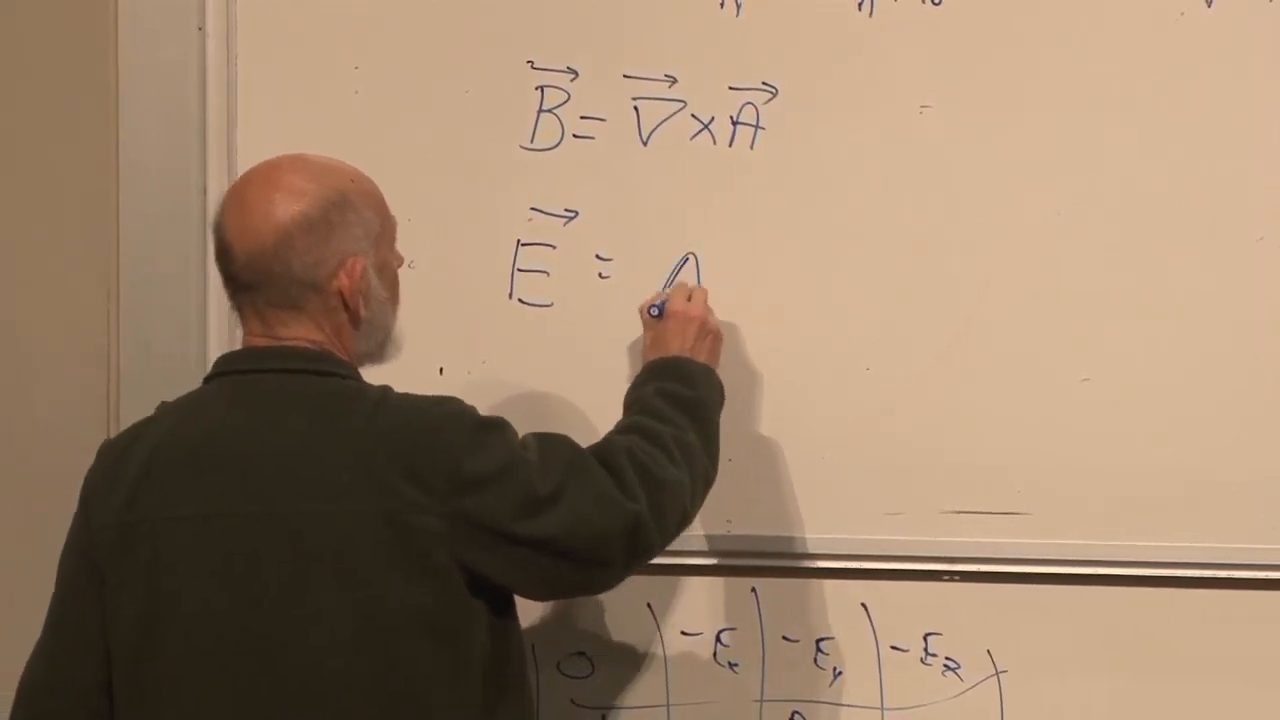
\includegraphics[width=\linewidth]{lecture_08_figure_03.png}\caption{칠판에 모아 쓴 전기장의 벡터 퍼텐셜 식과 자기장의 회전.}\par\smallskip
\textit{강의 화면: 00:14:00.}\end{figure}

\subsection{성분 배열}

첫 번째 텐서 첨자를 행, 두 번째 첨자를 열의 표지로 삼고, 순서는 \(0,x,y,z\)로 하자. 그러면
\begin{equation}
F_{\mu\nu}
=
\begin{pmatrix}
0&E_x&E_y&E_z\\
-E_x&0&B_z&-B_y\\
-E_y&-B_z&0&B_x\\
-E_z&B_y&-B_x&0
\end{pmatrix}.
\label{eq:f-lower-matrix}
\end{equation}
시간--공간 혼합 성분에는 \(\mathbf E\)가 들어 있고, 공간 \(3\times3\) 블록에는 \(\mathbf B\)가 들어 있다. 아래쪽 삼각 영역은 위쪽 삼각 영역을 반사해 부호를 바꾼 것뿐이므로 새로운 정보가 아니다.

\begin{figure}[H]\centering
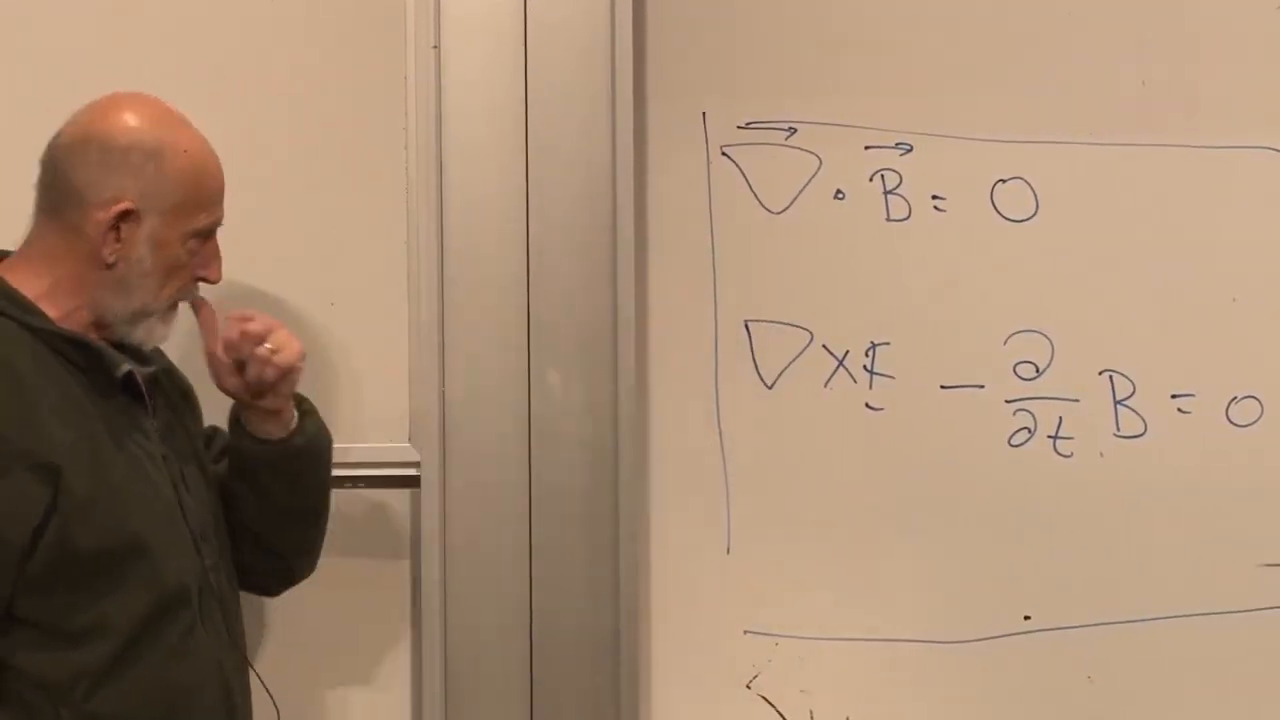
\includegraphics[width=\linewidth]{lecture_08_figure_04.png}\caption{전기 성분과 자기 공간 블록을 갖춘 아래 첨자 전자기장 텐서.}\par\smallskip
\textit{강의 화면: 00:17:15.}\end{figure}

두 첨자를 모두 올리면 모든 전기 성분의 부호가 바뀌고 자기 성분은 그대로다.
\begin{equation}
F^{\mu\nu}
=
\begin{pmatrix}
0&-E_x&-E_y&-E_z\\
E_x&0&B_z&-B_y\\
E_y&-B_z&0&B_x\\
E_z&B_y&-B_x&0
\end{pmatrix}.
\label{eq:f-upper-matrix}
\end{equation}
전기 성분에는 시간 첨자가 하나 있으므로 부호가 한 번 바뀐다. 자기 성분에는 공간 첨자가 두 개 있으므로 부호가 바뀌지 않는다.

\begin{classroomqa}\audiencequestion{행렬을 제대로 읽었다면 자기 성분에는 시간 첨자가 없는 건가요?}\lecturerresponse{그렇다. 자기 성분은 순수한 공간 블록에 놓인다. 전기 성분은 첫째 행과 첫째 열에 있는 시간--공간 혼합 성분이다. \lecturetimestamp{00:18:55}}\end{classroomqa}

\section{순수 자기장을 부스트하기}

\(x\)방향으로 부스트하고 \(c=1\)이라 하자.
\begin{align}
t'&=\gamma(t-vx),
&
x'&=\gamma(x-vt),
&
y'&=y,
&
z'&=z,
\end{align}
여기서
\begin{equation}
\gamma=\frac{1}{\sqrt{1-v^2}}.
\end{equation}
행렬로 쓰면 다음과 같다.
\begin{equation}
x'^\mu
=
\Lambda^\mu{}_\nu x^\nu,
\qquad
\Lambda^\mu{}_\nu
=
\begin{pmatrix}
\gamma&-\gamma v&0&0\\
-\gamma v&\gamma&0&0\\
0&0&1&0\\
0&0&0&1
\end{pmatrix}.
\label{eq:x-boost}
\end{equation}

\begin{classroomqa}\audiencequestion{부스트 행렬에서 마이너스 부호가 빠진 것 아닌가요?}\lecturerresponse{그렇다. 시간--공간 비대각 성분에는 \(t'=\gamma(t-vx)\)와 \(x'=\gamma(x-vt)\)에 필요한 마이너스 부호가 들어간다. 장을 변환하기 전에 이를 바로잡는다. \lecturetimestamp{00:23:50}}\end{classroomqa}

\begin{figure}[H]\centering
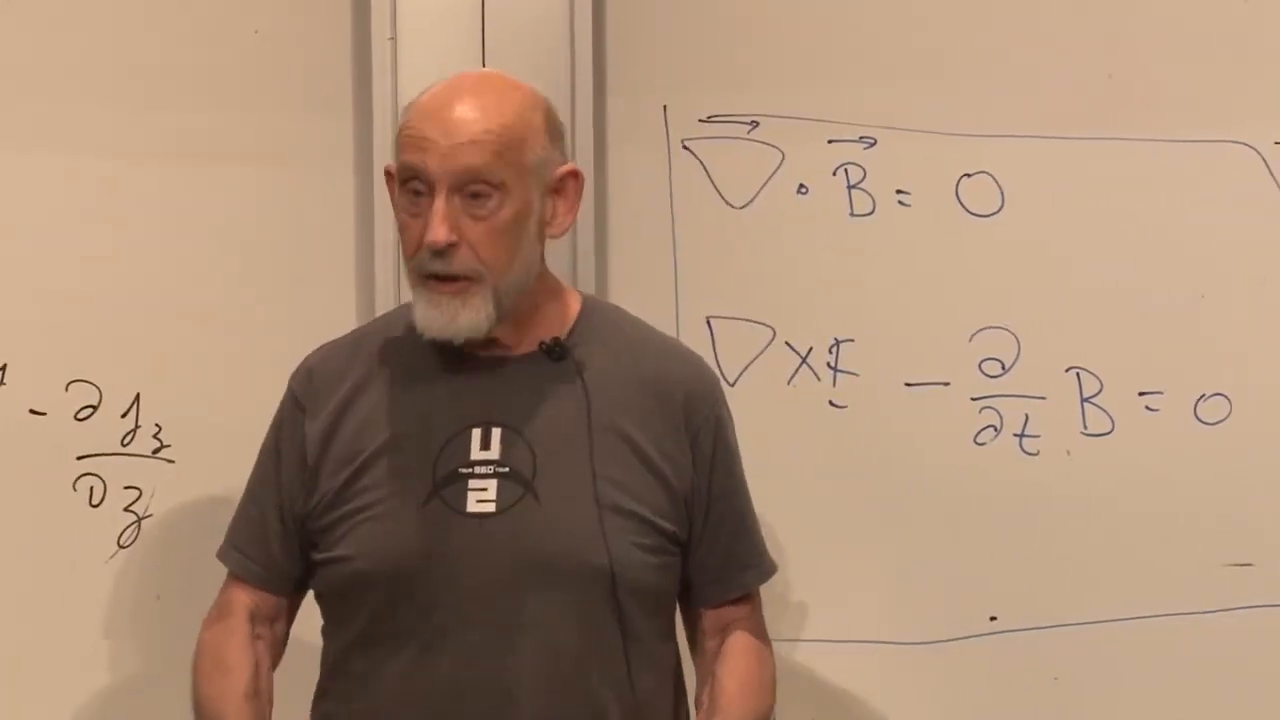
\includegraphics[width=\linewidth]{lecture_08_figure_05.png}\caption{\(x\)축을 따른 운동에 대한 수정된 로런츠 부스트 행렬.}\par\smallskip
\textit{강의 화면: 00:24:00.}\end{figure}

모든 위 첨자 텐서 지수는 위 첨자 벡터 지수처럼 변환한다. 따라서
\begin{equation}
F'^{\mu\nu}
=
\Lambda^\mu{}_\sigma
\Lambda^\nu{}_\tau
F^{\sigma\tau}.
\label{eq:f-boost-law}
\end{equation}
반복된 \(\sigma\)와 \(\tau\)는 더미 지수다. 지수가 더 많은 텐서라면 지수마다 변환 행렬 하나씩이 나타난다.

\begin{figure}[H]\centering
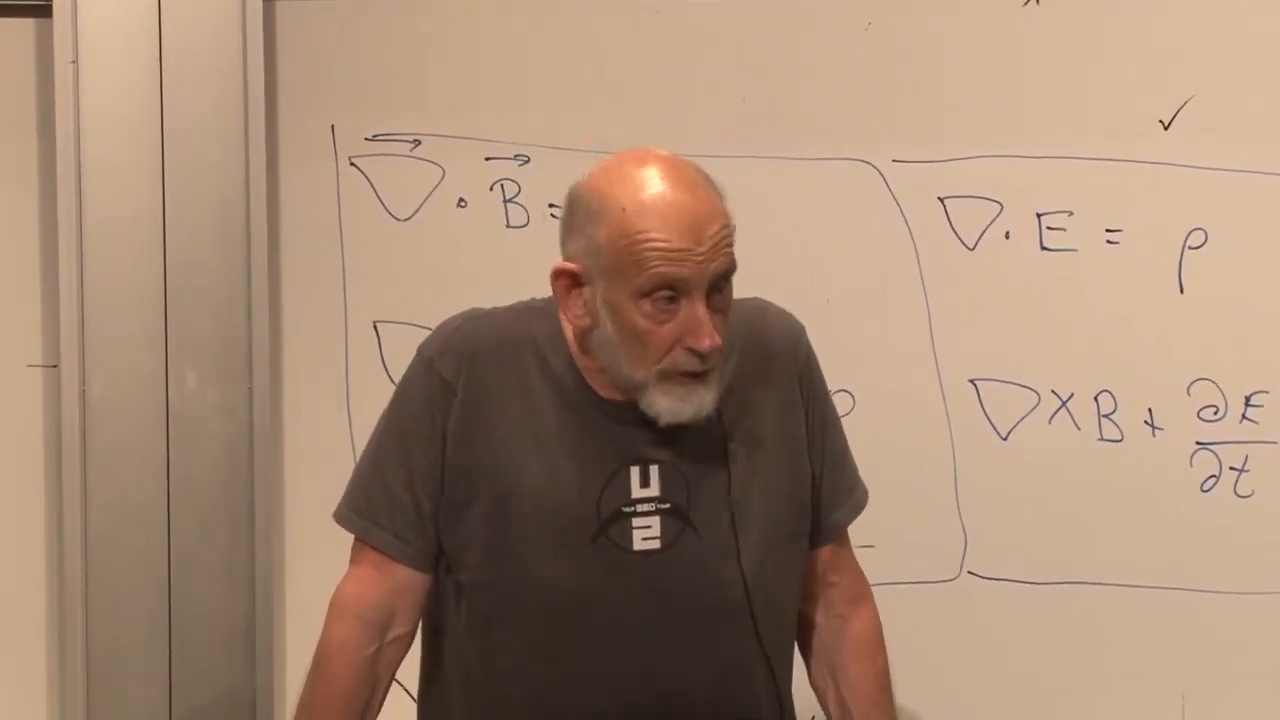
\includegraphics[width=\linewidth]{lecture_08_figure_06.png}\caption{랭크 2 로런츠 변환 법칙. 장 텐서의 각 지수마다 부스트 행렬 하나가 곱해진다.}\par\smallskip
\textit{강의 화면: 00:26:40.}\end{figure}

\subsection{전기장 성분으로 바뀌는 성분}

프라임이 붙지 않은 기준계에 자기장 \(B_y\)만 있다고 하자. ~\eqref{eq:f-upper-matrix}의 규약에 따르면 관련된 독립 성분은
\begin{equation}
F^{xz}=-B_y.
\end{equation}
프라임이 붙은 전기장의 \(z\)성분을 나타내는 혼합 성분 \(F'^{0z}\)을 구하려 한다. \eqref{eq:f-boost-law}에서
\begin{align}
F'^{0z}
&=
\Lambda^0{}_\sigma
\Lambda^z{}_\tau F^{\sigma\tau}
\\
&=
\Lambda^0{}_x\Lambda^z{}_zF^{xz}
\\
&=
(-\gamma v)(1)(-B_y)
=
\gamma vB_y.
\end{align}을 얻는다. 이 규약에서는 \(F'^{0z}=-E'_z\)이므로
\begin{equation}
E'_z=-\gamma vB_y.
\label{eq:boosted-electric-field}
\end{equation}
부호는 정해 둔 축과 장의 규약에 따라 달라진다. 계산에서 변하지 않는 핵심은
\begin{equation}
\lvert E'_z\rvert
=
\gamma\lvert vB_y\rvert
\ne0.
\end{equation}
원래 장에는 독립적인 자기 성분이 하나뿐이므로 이중 합은 이 항 하나만 남는다.

\begin{figure}[H]\centering
\includegraphics[width=\linewidth]{lecture_08_figure_07.png}\caption{부스트 뒤에 선택한 텐서 성분. 원래 자기 성분에 곱해지는 인자는 \(\gamma v\)이다.}\par\smallskip
\textit{강의 화면: 00:32:30.}\end{figure}

프라임이 붙은 기준계가 전하와 함께 움직이도록 하자. 그러면 전하는 정지하므로 전하가 받는 힘에서 자기적 부분 \(q\,\mathbf v'\times\mathbf B'\)은 없다. 그렇다고 힘이 사라지는 것은 아니다. 힘은 \(q\mathbf E'\)이다. 실험실 관찰자가 보는 자기력과 전하와 함께 움직이는 관찰자가 보는 전기력은 동일한 사건에 대한 두 가지 설명이다.

이것이 아인슈타인 논문 첫 문단의 수수께끼에 대한 답이다. 이 질문에 강의에서 대략 처음 40분을 썼다. 역사적으로 보면 아인슈타인은 이 문제를 훨씬 더 오래 붙들고 있었다는 농담도 있다. 전기장과 자기장이 섞인다는 구호를 하나의 명시적인 텐서 성분으로 보여 주므로, 이 계산에 시간을 들일 만하다.

\section{맥스웰 방정식: 항등식과 동역학}

이제 전하에 작용하는 힘에서 장 방정식으로 넘어가자. 다음 강의에서는 작용으로부터 장 방정식을 유도할 것이다. 여기서는 우선 방정식들을 제시하고, 서로 다른 두 가지 논리적 역할을 이해하며, 항등식에 근거한 절반을 공변 형식으로 표현하는 것이 목적이다.

\begin{classroomqa}\audiencequestion{이 방정식들은 이미 유도하지 않았나요?}\lecturerresponse{주어진 전자기장 속에서 대전 입자의 운동 방정식은 유도했다. 맥스웰 방정식은 전하와 전류에 대한 장의 반응을 포함하여 장 자체의 운동 방정식을 나타낸다. \lecturetimestamp{00:35:10}}\end{classroomqa}

\begin{classroomqa}\audiencequestion{맥스웰 방정식은 몇 개인가요?}\lecturerresponse{성분 방정식으로는 스칼라 방정식이 8개다. 벡터 표기법에서는 이를 스칼라 방정식 2개와 3성분 벡터 방정식 2개로 묶어, 관례적으로 맥스웰 방정식 4개라고 부른다. \lecturetimestamp{00:35:24}}\end{classroomqa}

\(c=1\)이고 통상적인 진공 상수들이 전하와 전류의 정의에 흡수된 단위를 계속 사용한다. 8개 성분 방정식 가운데 4개는 정의 \(F=dA\)에서 따른다. 이들은 운동학적 항등식이다. 나머지 4개는 동역학적 방정식이며, 장의 작용이 달라지면 함께 달라질 수 있다.

\subsection{기본 벡터 연산 세 가지}

미분 가능한 3차원 벡터장 \(\mathbf A\)에 대해
\begin{align}
(\boldsymbol\nabla\times\mathbf A)_x
&=
\partial_yA_z-\partial_zA_y,
\\
\boldsymbol\nabla\cdot\mathbf A
&=
\partial_xA_x+\partial_yA_y+\partial_zA_z.
\end{align}
나머지 회전 성분은 \(x\to y\to z\to x\)를 순환 치환해 얻는다. 스칼라장 \(s\)에 대해서는
\begin{equation}
\boldsymbol\nabla s
=
(\partial_xs,\partial_ys,\partial_zs).
\end{equation}
따라서 회전은 벡터이고, 발산은 스칼라이며, 기울기는 벡터다.

\begin{classroomqa}\audiencequestion{회전과 발산의 정의를 처음부터 전부 복습할 필요가 있나요?}\lecturerresponse{성분별 정의는 적어 두었지만 나머지 성분을 모두 전개할 필요는 없다. 좌표 표지를 순환시키면 얻을 수 있다. \lecturetimestamp{00:37:32}}\end{classroomqa}

매끄러운 함수의 편미분은 교환 가능하므로 다음 두 항등식이 성립한다.
\begin{align}
\boldsymbol\nabla\cdot
(\boldsymbol\nabla\times\mathbf A)
&=0,
\label{eq:div-curl}
\\
\boldsymbol\nabla\times
(\boldsymbol\nabla s)
&=\mathbf0.
\label{eq:curl-grad}
\end{align}

\begin{classroomqa}
\audiencequestion{컬의 발산이 사라짐을 보이는 성분별 증명을 전부 써 볼까요?}
\lecturerresponse{수강생들은 쓰지 않기로 한다. 성분을 전개하면 \(\partial_x\partial_yA_z\)와 \(-\partial_y\partial_xA_z\) 같은 항들이 쌍으로 나타나며, 미분 순서를 바꿀 수 있으므로 서로 상쇄된다. \lecturetimestamp{00:40:13}}
\end{classroomqa}

\begin{figure}[H]\centering
\includegraphics[width=\linewidth]{lecture_08_figure_08.png}\caption{맥스웰 방정식의 절반을 얻는 데 쓰인 회전의 발산과 기울기의 회전 항등식.}\par\smallskip
\textit{강의 화면: 00:41:40.}\end{figure}

\subsection{벡터 퍼텐셜에서는 자기 원천이 생기지 않는다}

~\eqref{eq:b-from-a}의 발산을 취하면
\begin{equation}
\boldsymbol\nabla\cdot\mathbf B
=
\boldsymbol\nabla\cdot
(\boldsymbol\nabla\times\mathbf A)
=0.
\label{eq:div-b-zero}
\end{equation}
운동 방정식은 사용하지 않았다. 이 결과는 퍼텐셜 표현과 매끄러운 편미분만으로 따른다.

\begin{figure}[H]\centering
\includegraphics[width=\linewidth]{lecture_08_figure_09.png}\caption{자기장의 발산이 회전의 발산으로 환원된다.}\par\smallskip
\textit{강의 화면: 00:43:05.}\end{figure}

\begin{classroomqa}\audiencequestion{전기장의 발산은 무엇인가요?}\lecturerresponse{사용하는 단위계에서는 전하 밀도, 즉 \(\boldsymbol\nabla\cdot\mathbf E=\rho\)이다. 점전하는 전기력선이 원천에서 퍼져 나가는 대표적인 예다. \lecturetimestamp{00:43:20}}\end{classroomqa}

기초적인 수준에서 보면 ~\eqref{eq:div-b-zero}은 자기 전하 밀도가 없다는 뜻이다. 매끄럽고 전역적으로 정의된 벡터 퍼텐셜로는 자기 단극자 원천을 만들 수 없다. 다만 이 진술에는 나중에 조건을 덧붙여야 한다. 겹치는 패치에서 정의된 퍼텐셜이나 특이한 게이지 선택을 사용하면 자기 단극자를 기술할 수 있다. 강의에서는 이 정교한 논의를 뒤로 미룬다.

\subsection{전기 퍼텐셜에서 얻는 패러데이 방정식}

식~\eqref{eq:e-from-a}을 삼차원 벡터 표기로 쓰면 다음과 같다.
\begin{equation}
\mathbf E
=
\frac{\partial\mathbf A}{\partial t}
-\boldsymbol\nabla A_0.
\label{eq:e-vector-potential}
\end{equation}
\(A_0\)는 사차원 벡터의 성분이지만, 통상적인 공간 회전에서는 스칼라이다. 컬을 취하면 다음과 같다.
\begin{align}
\boldsymbol\nabla\times\mathbf E
&=
\boldsymbol\nabla\times
\frac{\partial\mathbf A}{\partial t}
-
\boldsymbol\nabla\times
(\boldsymbol\nabla A_0)
\\
&=
\frac{\partial}{\partial t}
(\boldsymbol\nabla\times\mathbf A)
\\
&=
\frac{\partial\mathbf B}{\partial t}.
\end{align}
공간 컬은 시간 미분과 교환되며, 기울기의 컬은 사라진다.

\begin{figure}[H]\centering
\includegraphics[width=\linewidth]{lecture_08_figure_10.png}\caption{자기장의 회전과 전기 퍼텐셜 식, 그리고 회전 계산의 시작을 함께 적은 칠판 모습.}\par\smallskip
\textit{강의 화면: 00:47:45.}\end{figure}

따라서 비동차항이 없는 성분 방정식 4개는 다음과 같다.
\begin{align}
\boldsymbol\nabla\cdot\mathbf B&=0,
\label{eq:homogeneous-div}
\\
\boldsymbol\nabla\times\mathbf E
-\frac{\partial\mathbf B}{\partial t}
&=\mathbf0.
\label{eq:homogeneous-curl}
\end{align}
첫째는 스칼라 방정식 하나이고, 둘째는 3성분 벡터 방정식이다.

\begin{figure}[H]\centering
\includegraphics[width=\linewidth]{lecture_08_figure_11.png}\caption{퍼텐셜의 정의에서 직접 얻은 원천이 없는 맥스웰 방정식 쌍.}\par\smallskip
\textit{강의 화면: 00:48:45.}\end{figure}

\subsection{동역학에 해당하는 절반}

나머지 방정식은 다음과 같다.
\begin{align}
\boldsymbol\nabla\cdot\mathbf E&=\rho,
\label{eq:gauss-electric}
\\
\boldsymbol\nabla\times\mathbf B
+\frac{\partial\mathbf E}{\partial t}
&=-\mathbf J.
\label{eq:ampere-maxwell}
\end{align}
이 방정식들은 \(F=dA\)에서 따르지 않는다. 원천이 어떻게 장을 만들고 변화시키는지를 기술하며, 다음 강의에서 전자기 작용으로부터 유도할 것이다. 전류 항의 마이너스 부호는 이미 정한 규약으로 결정된다. 즉 \(F_{0i}=E_i\), \(F_{ij}=\epsilon_{ijk}B_k\), 그리고 \(\partial_\mu F^{\mu\nu}=J^\nu\)이다. 강의 중 칠판에는 처음에 \(\mathbf J\)가 이 마이너스 부호 없이 우변에 적혔다. 그 결과 전하 보존 법칙과 맞지 않는 점을 다음 강의에서 알아차리고 바로잡는다.

\begin{classroomqa}\audiencequestion{회전 방정식 우변에는 어떤 종류의 물리량이 있나요?}\lecturerresponse{좌변이 3차원 벡터이므로 우변도 3차원 벡터이며, 이를 전류 밀도 \(\mathbf J\)라고 한다. 가우스 방정식 우변은 3차원 스칼라 전하 밀도 \(\rho\)다. \lecturetimestamp{00:50:36}}\end{classroomqa}

\begin{figure}[H]\centering
\includegraphics[width=\linewidth]{lecture_08_figure_12.png}\caption{항등식에 근거한 쌍과 원천이 있는 동역학적 쌍으로 묶어 쓴 맥스웰 방정식 4개.}\par\smallskip
\textit{강의 화면: 00:50:40.}\end{figure}

\section{시공간의 흐름으로서의 전하와 전류}

이제 기호 \(\rho\)와 \(\mathbf J\)에 기하학적 의미를 부여해야 한다. 전하 밀도는 단위 부피당 전하이고, 전류 밀도는 단위 시간 동안 방향이 정해진 면을 통과하는 전하량이다. 강의에서는 두 양을 모두 세계선에서 출발해 설명한다. 그래야 나중에 이들이 하나의 4-벡터로 합쳐지는 일이 우연처럼 보이지 않을 것이다.

\subsection{옆 칠판에 보이는 내용에 관한 수업 중 여담}

세계선을 그리기 전에 옆 강의실에 보이는 방정식들 때문에 잠시 수업에서 벗어나 이야기를 나눈다. 곧 개설될 강좌에서는 양자장론과 현대 수학과의 관련성을 이해하는 데 필요한 배경을 얻고 싶어 하는 수학 교수진에게 양자역학을 소개할 예정이었다. 어려움은 양쪽 모두에 있다. 물리학자는 암묵적으로 익힌 물리학적 사고방식을 명시적으로 설명해야 하고, 수학자는 형식적 구조가 무엇을 기술하도록 고안되었는지 배워야 한다.

\begin{classroomqa}\audiencequestion{그 강의는 누가 힘들어할까요?}\lecturerresponse{아마 양쪽 모두일 것이다. 익숙하지 않은 청중을 가르치는 물리학자와, 형식론의 바탕이 되는 물리학적 사고방식에 부딪히는 수학자 모두 그렇다. 그래도 그 강의는 재미있을 것으로 예상된다. 이어서 수업은 전하와 전류로 돌아간다. \lecturetimestamp{00:53:20}}\end{classroomqa}

\subsection{전하 밀도}

시간을 세로축으로 그리고, 나머지 축은 3차원 공간을 나타내도록 하자. 대전 입자들은 세계선을 그린다. 한 시각을 고정하고 부피가 \(\Delta V\)인 작은 공간 정육면체를 그 세계선 다발에 걸쳐 놓은 뒤, 그 안에 있는 입자들의 전하를 모두 더한다. 전하 밀도는
\begin{equation}
\rho(t,\mathbf x)
=
\lim_{\Delta V\to0}
\frac{\Delta Q}{\Delta V}.
\label{eq:charge-density}
\end{equation}
칠판에 그린 2차원 정사각형은 3차원 정육면체를 나타낸다. 네 차원을 평면 칠판에 그릴 수 없어 공간 방향 하나를 생략했을 뿐이다.

\begin{figure}[H]\centering
\includegraphics[width=\linewidth]{lecture_08_figure_13.png}\caption{작은 공간 셀을 통과하는 대전 입자들의 세계선. \(\rho=\Delta Q/\Delta V\).}\par\smallskip
\textit{강의 화면: 00:57:20.}\end{figure}

\subsection{전류 밀도}

시공간 셀을 옆으로 돌려 보자. \(J_x\)를 정의하려면 \(yz\)면 안에 놓인 작은 창의 넓이 \(\Delta A_x\)를 택한다. 이 창은 \(x\)축에 수직이다. \(\Delta t\) 동안 음의 \(x\) 쪽에서 양의 \(x\) 쪽으로 통과하는 순전하량을 센다.
\begin{equation}
J_x
=
\lim_{\Delta A_x,\Delta t\to0}
\frac{\Delta Q_x}{\Delta A_x\,\Delta t}.
\label{eq:jx-window}
\end{equation}
방향이 부호를 정한다. \(y\)와 \(z\)에 수직인 창으로도 같은 방식으로 \(J_y\)와 \(J_z\)을 정의한다.

칠판 그림은 그리기 어려운 점을 그대로 드러낸다. \(yz\)면에 놓인 창은 벽의 창보다 천장에 난 창처럼 보인다. 한 번에 표시할 수 있는 축보다 관련된 축이 더 많기 때문이다. 스케치는 명확하지 않아도 불변인 정의 자체는 모호하지 않다.

\begin{classroomqa}\audiencequestion{그림에서 창은 천장에 나 있는 건가요?}\lecturerresponse{방에 비유하자면 그렇다. 중요한 것은 창의 면이 \(x\) 방향에 수직이라는 점이다. 넓이가 \(yz\)인 면은 그 면을 통과하는 \(x\) 방향 전류를 잰다. \lecturetimestamp{00:59:38}}\end{classroomqa}

\begin{figure}[H]\centering
\includegraphics[width=\linewidth]{lecture_08_figure_14.png}\caption{횡방향 창을 통과하는 전하 전류. \(J_x=\Delta Q/(\Delta A\,\Delta t)\).}\par\smallskip
\textit{강의 화면: 01:01:40.}\end{figure}

\begin{figure}[H]\centering
\includegraphics[width=\linewidth]{lecture_08_figure_15.png}\caption{세 공간축에 수직인 창을 통과하는 전하량으로 정의한 전류의 세 성분.}\par\smallskip
\textit{강의 화면: 01:02:40.}\end{figure}

네 물리량은 서로 짝을 이루는 방식으로 정의된다. 한순간의 공간 부피는 시간축에 수직인 초곡면이므로, \(\rho\)은 시간축에 수직인 창을 통과하는 전하 흐름이다. \(J_i\)는 공간축에 수직인 창들을 통과하는 흐름이다.

\begin{classroomqa}\audiencequestion{네 성분은 시간 방향의 흐름 하나와 공간 방향의 흐름 세 개인가요?}\lecturerresponse{그렇게 생각하면 정확하다. 공간 부피는 시간축에 수직인 창이고, 세 횡방향 면은 각각 \(x\), \(y\), \(z\)에 수직인 창이다. 이 네 가지 플럭스는 함께 묶인다. \lecturetimestamp{01:04:14}}\end{classroomqa}

이로부터 반변 4-전류를 생각할 수 있다.
\begin{equation}
J^\mu
=
(\rho,J_x,J_y,J_z).
\label{eq:four-current}
\end{equation}

\begin{classroomqa}\audiencequestion{계량은 어디에 들어가나요? 이 전류는 공변인가요, 반변인가요?}\lecturerresponse{여기서 정의한 \(\rho\)과 세 \(J_i\)는 \(J^\mu\)의 성분이며, 위 첨자를 가진 반변 4-벡터를 이룬다. \(J_\mu\)가 필요하면 계량을 이용해 지수를 내린다. 공변적인 맥스웰 방정식의 표현을 보면 위 첨자를 택한 것이 왜 자연스러운지 알 수 있다. \lecturetimestamp{01:04:48}}\end{classroomqa}

\section{휴식 시간의 막간: 블랙홀 근처의 신호}

예정된 휴식 시간에 질문은 앞서 나눈 블랙홀 이야기로 이어진다. 전기역학에서 벗어난 여담이지만, 수업 중 상당한 토론이 오갔고 서로 다른 관찰자의 설명을 구분하는 같은 사고방식을 보여 준다.

\begin{classroomqa}\audiencequestion{멀리 떨어진 관찰자에게 낙하하는 물체가 사건의 지평선 근처에서 느려지는 것으로 보인다면, 블랙홀은 과거에 낙하한 모든 물체로 덮여 보이나요?}\lecturerresponse{슈바르츠실트 좌표 시간으로 기술하면 고전적인 낙하 물체는 점근적으로 사건의 지평선에 접근하는 것으로 보인다. 물질이 차례로 쌓여 지평선 근처의 층이 점점 압축되는 모습을 그려 볼 수 있다. 하지만 관측 가능한 실제 신호는 점점 더 지연되고 적색편이되며 희미해진다. 보통의 국소 진동수로 방출된 빛은 처음에는 가시광선으로 도착하고, 이어 적외선, 마이크로파, 전파로 도착하며, 광자 하나하나의 에너지도 줄어든다. 현실적인 원거리 검출기라면 얼어붙은 듯한 밝은 물체를 영원히 보지는 못한다. 그것은 희미해져 어둠 속으로 사라진다.
\lecturetimestamp{01:06:11}}\end{classroomqa}

낙하하는 관찰자의 시계와 그 관찰자가 국소적으로 켠 손전등은 그 관찰자에게 평범하게 보인다. 원거리 관찰자의 설명이 달라지는 것은 진동수와 도착률이 적색편이되기 때문이다. 에너지와 대역폭이 유한하므로, 메시지 중 마지막으로 분해해 볼 수 있는 부분이 사실상 존재한다.

\begin{classroomqa}\audiencequestion{물체가 점근적으로 사건의 지평선에 접근하는 건가요?}\lecturerresponse{원거리 관찰자의 슈바르츠실트 좌표 설명에서는 그렇다. 양자역학적으로는 희미해지는 신호를 블랙홀의 호킹 복사와도 구별해야 한다. 충분히 늦은 시각에는 약하게 적색편이된 신호가 블랙홀 자체에서 나오는 복사의 배경에 묻혀 관측되지 않게 된다. \lecturetimestamp{01:09:24}}\end{classroomqa}

\begin{classroomqa}\audiencequestion{적색편이된 파장이 관측 가능한 우주의 크기를 넘어 커지면 어떻게 되나요?}\lecturerresponse{실제로는 그 한계에 도달하기 훨씬 전에 신호를 잃어버린다. 강의에서는 대략적인 호킹 복사 그림으로, 빛이 블랙홀을 가로지르는 시간마다 전형적인 양자 하나 정도가 방출된다고 설명한다.
\[
t_{\rm cross}\sim\frac{R_s}{c}.
\]
큰 블랙홀의 복사는 극도로 약하다. 적색편이된 낙하 신호는 우주론적 파장 한계에 이르기 훨씬 전에 검출 불가능해진다. \lecturetimestamp{01:09:50}}\end{classroomqa}

\begin{classroomqa}\audiencequestion{블랙홀의 수명 내내 통과 시간당 양자 하나 정도라는 방출률이 일정한가요?}\lecturerresponse{아니다. 증발하는 슈바르츠실트 블랙홀은 크기가 줄어들므로 통과 시간은 짧아지고 호킹 온도는 올라간다. 따라서 방출은 점점 빨라진다. 순간적인 반지름으로 나타낸 차원 추정은 여전히 유용하지만, 반지름은 일정하지 않다. 이에 따라 전형적인 호킹 파장은 증발이 진행될수록 짧아진다. \lecturetimestamp{01:11:42}}\end{classroomqa}

휴식 시간이 끝나고 재킷을 벗은 뒤, \(\rho\)와 \(\mathbf J\)로 돌아간다.

\section{전하의 국소 보존}

전하 보존을 다음과 같이만 말하고 싶은 유혹이 있다.
\begin{equation}
\frac{dQ_{\rm universe}}{dt}=0.
\end{equation}
하지만 이 진술은 너무 약하다. 전체 전하가 변하지 않은 채 실험실에서 사라진 전하가 즉시 알파 센타우리로, 혹은 더 멀리 떨어진 머리털자리 은하단으로 다시 나타날 수도 있기 때문이다. 그런 법칙은 실험적으로 검증할 여지가 거의 없다.

더 강한 진술은 국소적이다. 어떤 영역 안의 전하가 변할 수 있는 것은 그 영역의 경계를 통과할 때뿐이다. 한 점을 둘러싸는 작은 상자를 놓자. 상자 안의 전하가 증가하면 여섯 면을 통과하는 순전류가 안쪽을 향해야 한다. 전하가 감소하면 순전류는 바깥쪽을 향해야 한다.

\subsection{마주 보는 면을 통과하는 플럭스}

\(x\)에 수직인 두 면을 보자. 한 면의 안쪽 방향 기여는 \(x\)의 한 값에서 계산하고, 반대쪽 면의 기여는 그로부터 작은 거리만큼 떨어진 곳에서 계산한다. 두 기여의 차이를 상자 폭으로 나눈 값은 다음에 가까워진다.
\begin{equation}
-\partial_xJ_x.
\end{equation}
양의 \(J_x\)를 \(x\)가 증가하는 방향으로 흐르는 것으로 정의했지만 바깥쪽 플럭스는 상자 안의 전하를 감소시키므로 마이너스 부호가 붙는다. \(y\)면과 \(z\)면의 쌍도 마찬가지로 각각 \(-\partial_yJ_y\)와 \(-\partial_zJ_z\)를 기여한다. 따라서
\begin{equation}
\frac{\partial\rho}{\partial t}
=
-\partial_xJ_x-\partial_yJ_y-\partial_zJ_z
=
-\boldsymbol\nabla\cdot\mathbf J.
\end{equation}
동등하게,
\begin{equation}
\boxed{
\frac{\partial\rho}{\partial t}
+\boldsymbol\nabla\cdot\mathbf J=0
}.
\label{eq:continuity}
\end{equation}

\begin{figure}[H]\centering
\includegraphics[width=\linewidth]{lecture_08_figure_16.png}\caption{국소 보존 법칙 \(\dot\rho=-\boldsymbol\nabla\cdot\mathbf J\)과, 경계면의 전류를 통해 그 법칙이 나타나는 작은 상자.}\par\smallskip
\textit{강의 화면: 01:20:45.}\end{figure}

통상 이 식을 연속 방정식이라고 부른다. 강의에서는 \emph{국소 보존}이라는 이름을 선호한다. 연속이라는 말은 수학적 매끄러움 조건을 떠올리게 할 수 있지만, 물리적 내용은 전류가 그 사이를 흐르지 않는 한 전하가 여기서 사라졌다가 저기서 다시 나타날 수 없다는 것이다.

\subsection{맥스웰이 변위 전류를 도입해야 했던 이유}

식~\eqref{eq:continuity}은 맥스웰 방정식에 독립적으로 추가되는 식이 아니다. 가우스 법칙을 시간에 대해 미분하고 앙페르--맥스웰 법칙의 발산을 취하면 다음과 같다.
\begin{align}
\frac{\partial\rho}{\partial t}
&=
\boldsymbol\nabla\cdot
\frac{\partial\mathbf E}{\partial t},
\\
-\boldsymbol\nabla\cdot\mathbf J
&=
\boldsymbol\nabla\cdot
(\boldsymbol\nabla\times\mathbf B)
+
\boldsymbol\nabla\cdot
\frac{\partial\mathbf E}{\partial t}
\\
&=
\boldsymbol\nabla\cdot
\frac{\partial\mathbf E}{\partial t}.
\end{align}
따라서 두 좌변은 같으며, 이에 따라 \(\partial_t\rho=-\boldsymbol\nabla\cdot\mathbf J\)가 되고, 이는 정확히 식~\eqref{eq:continuity}이다. 구조적으로 중요한 점은 전하 보존과 발산 관계가 서로 양립하려면 \(\mathbf E\), 즉 변위 전류 항의 시간 미분이 꼭 필요하다는 것이다.

\begin{classroomqa}
\audiencequestion{전하를 포함하는 두 맥스웰 방정식이 어디서 나오는지는 아직 보이지 않았죠?}
\lecturerresponse{그렇다. 이 방정식들은 다음에 작용으로부터 유도할 동역학적 목표다. 정자기 컬 법칙은 맥스웰 이전부터 알려져 있었고, 맥스웰의 결정적인 시간 의존성 추가 항은 변위 전류였다. 이 항이 있어야 장 방정식이 국소 전하 보존과 양립한다. \lecturetimestamp{01:23:15}}
\end{classroomqa}

발산을 상세히 계산하는 과정은 강의에서 연습문제로 남겨 두지만, 그 결론은 선택 사항이 아니다. 맥스웰 방정식은 전하 보존을 요구한다.

\section{4-전류와 그 발산}

식~\eqref{eq:continuity}을 성분별로 쓰면 다음과 같다.
\begin{equation}
\frac{\partial\rho}{\partial t}
+
\frac{\partial J_x}{\partial x}
+
\frac{\partial J_y}{\partial y}
+
\frac{\partial J_z}{\partial z}
=0.
\label{eq:continuity-components}
\end{equation}

\begin{figure}[H]
\centering
\includegraphics[width=\linewidth]{lecture_08_figure_17.png}
\caption{국소 전하 보존을 시간 미분 하나와 공간 미분 세 개로 전개한 식.}
\par\smallskip
\textit{강의 시각: 01:25:40.}
\end{figure}

\(J^\mu\)를 식~\eqref{eq:four-current}으로 정의하면, 네 항은 하나의 수축으로 표현된다.
\begin{equation}
\boxed{\partial_\mu J^\mu=0}.
\label{eq:four-current-conservation}
\end{equation}
\(\partial_\mu\)의 아래 첨자는 \(J^\mu\)의 위 첨자와 수축하므로, 그 결과는 로런츠 스칼라이다. 기하학적 창 구성은 이미 이러한 변환 법칙을 시사했다. \(\rho\)와 전류의 세 성분은 같은 전하 흐름을 네 방향에서 본 것이다.

\begin{figure}[H]
\centering
\includegraphics[width=\linewidth]{lecture_08_figure_18.png}
\caption{성분 \((\rho,J_x,J_y,J_z)\)을 \(J^\mu\)로 모아 4-기울기와 수축한다.}
\par\smallskip
\textit{강의 시각: 01:27:10.}
\end{figure}

\begin{classroomqa}
\audiencequestion{\(\rho\)의 시간 미분은 언제 편미분이 되었나요?}
\lecturerresponse{처음부터 편미분이었다. 우리는 공간 상자를 고정해 두고 시간에 따라 그 안의 전하 밀도가 어떻게 변하는지 묻는다. 움직이는 궤적을 따라가는 것이 아니므로, 여기서 \(\dot\rho\)는 고정된 \(x,y,z\)에서의 \(\partial\rho/\partial t\)를 뜻한다.
\lecturetimestamp{01:28:20}}
\end{classroomqa}

\section{공변 형식으로 쓴 동차 방정식}

이제 필요한 대상들이 갖추어졌다.
\begin{itemize}
\item \(\mathbf E\)와 \(\mathbf B\)는 반대칭 텐서 \(F_{\mu\nu}\)의 서로 독립인 여섯 성분이고,
\item \(\rho\)와 \(\mathbf J\)는 \(J^\mu\)의 네 성분이며,
\item 국소 보존은 스칼라 방정식 \(\partial_\mu J^\mu=0\)이다.
\end{itemize}
이번 강의에서 남은 과제는 동차 맥스웰 방정식 쌍, 즉 식~\eqref{eq:homogeneous-div}과 식\eqref{eq:homogeneous-curl}을 하나의 텐서 방정식으로 쓰는 것이다.

\subsection{순환 미분}

답은 다음과 같다.
\begin{equation}
\boxed{
\partial_\sigma F_{\nu\tau}
+
\partial_\nu F_{\tau\sigma}
+
\partial_\tau F_{\sigma\nu}
=0
}.
\label{eq:bianchi}
\end{equation}
세 항에서는 미분 지수와 장 텐서의 두 지수가 순환적으로 자리를 바꾼다. 이를 흔히 다음과 같이 줄여 쓴다.
\begin{equation}
\partial_{[\sigma}F_{\nu\tau]}=0,
\end{equation}
여기서 대괄호는 반대칭화를 뜻한다.

\begin{figure}[H]
\centering
\includegraphics[width=\linewidth]{lecture_08_figure_19.png}
\caption{동차 맥스웰 방정식들을 하나로 묶어 나타내는 순환형 세 지표 방정식.}
\par\smallskip
\textit{강의 시점: 01:33:20.}
\end{figure}

\subsection{세 지수가 모두 공간 지수인 경우}

다음과 같이 두자.
\begin{equation}
(\sigma,\nu,\tau)=(x,y,z).
\end{equation}
그러면 다음과 같다.
\begin{align}
0
&=
\partial_xF_{yz}
+
\partial_yF_{zx}
+
\partial_zF_{xy}
\\
&=
\partial_xB_x+\partial_yB_y+\partial_zB_z
\\
&=
\boldsymbol\nabla\cdot\mathbf B.
\end{align}
따라서 식~\eqref{eq:bianchi}에서 세 지수가 모두 공간 지수인 성분은 자기장의 발산이 없다는 조건과 정확히 일치한다.

\begin{figure}[H]
\centering
\includegraphics[width=\linewidth]{lecture_08_figure_20.png}
\caption{순환 항등식에서 모든 지표가 공간 지표인 성분을 \(\partial_xB_x+\partial_yB_y+\partial_zB_z=0\)로 줄인 식.}
\par\smallskip
\textit{강의 시점: 01:35:30.}
\end{figure}

\subsection{시간 지수 하나}

예를 들어 다음을 택하자.
\begin{equation}
(\sigma,\nu,\tau)=(y,x,0).
\end{equation}
그러면 식~\eqref{eq:bianchi}은 전기장 성분의 공간 미분 두 개와 자기장 성분의 시간 미분 하나를 결합한다.
\begin{equation}
\partial_yF_{x0}
+
\partial_xF_{0y}
+
\partial_0F_{yx}
=0.
\end{equation}
식~\eqref{eq:f-lower-matrix}의 행렬을 이용하면 이는 다음 방정식의 한 성분이다.
\begin{equation}
\boldsymbol\nabla\times\mathbf E
-\frac{\partial\mathbf B}{\partial t}
=\mathbf0,
\end{equation}
상대 부호는 반대칭성에 의해 정해진다. 공간 지수의 다른 조합을 택하면 컬 방정식의 나머지 두 성분을 얻는다.

\begin{figure}[H]
\centering
\includegraphics[width=\linewidth]{lecture_08_figure_21.png}
\caption{파라데이 방정식의 한 성분을 얻는 시간 지표 하나와 공간 지표 둘의 성분 확인.}
\par\smallskip
\textit{강의 시점: 01:38:20.}
\end{figure}

직접 증명할 수도 있다. 식~\eqref{eq:field-tensor-definition}을 식~\eqref{eq:bianchi}에 대입하면 2계 미분 항 여섯 개가 나타나며, 편미분끼리 교환되므로 쌍을 이루어 상쇄된다. 이는 발산의 컬과 기울기의 컬에 관한 항등식을 4차원으로 확장한 것이다.

\begin{classroomqa}
\audiencequestion{비앙키라는 이름에 \(h\)가 들어가나요?}
\lecturerresponse{그렇다. 이 순환 방정식은 전자기 비앙키 항등식이며, 일반 상대성이론에도 나타나는 기하학적 항등식의 특수한 경우다. 더 깊은 기하학적 해석은 뒤로 미룬다.
\lecturetimestamp{01:40:28}}
\end{classroomqa}

\subsection{쓰인 성분은 64개인데 방정식은 네 개뿐인 이유}

각각 네 가지 값을 가질 수 있는 세 지표는 \(4^3=64\)개의 방정식을 만드는 듯하다. 반대칭성으로 중복을 제거하면 다음과 같다.
\begin{itemize}
\item 두 지표가 같으면 순환식은 항등적으로 사라진다.
\item 세 지표가 모두 서로 다르면, 순열에 따라 부호만 달라질 뿐 같은 방정식이 나온다.
\item 사차원에는 서로 다른 지표 세 개로 이루어진 순서 없는 조합이 \(\binom{4}{3}=4\)개뿐이다.
\end{itemize}
모든 지표가 서로 다른 순서 있는 세 지표의 배열은 \(24\)개이며, 이는 각각 여섯 순열로 이루어진 네 묶음으로 나뉜다. 나머지 \(40\)개의 배열은 사라진다. 서로 독립인 네 방정식은 자기장 발산 방정식 하나와 패러데이 방정식의 세 성분이다.

\begin{classroomqa}
\audiencequestion{장 텐서에는 서로 독립인 성분이 여섯 개뿐인데, 3지수 식에는 방정식이 64개나 있는 것 같습니다. 왜 네 개만 남나요?}
\lecturerresponse{지수가 반복되면 0이 되고, 서로 다른 세 지수의 순열은 부호만 다른 같은 관계를 나타낸다. 따라서 겉보기에는 64개인 성분이 서로 독립인 네 방정식으로 줄어든다.
\lecturetimestamp{01:41:58}}
\end{classroomqa}

식~\eqref{eq:bianchi}은 텐서 방정식임이 명백하므로 로런츠 공변적이다. 매끄러운 단일 퍼텐셜 기술에서는 자기 전하 밀도와 자기 전류가 모두 없다는 뜻이기도 하다. 동역학적 원천 항 방정식 쌍은 강의에서 도달한 바로 그 지점에서 남겨 둔다. 그 공변 방정식과 작용으로부터의 유도는 다음 시간에 다룬다.

\section{쌍대성과 자기 홀극 문제}

마지막 질문은 전기 원천과 자기 원천 사이의 겉보기 비대칭으로 돌아간다. 진공에서 맥스웰 방정식은 전기--자기 쌍대성 회전을 허용한다.
\begin{equation}
\mathbf E\longrightarrow\mathbf B,
\qquad
\mathbf B\longrightarrow-\mathbf E.
\label{eq:duality-quarter-turn}
\end{equation}
이는 축이 \(\mathbf E\)와 \(\mathbf B\)인 추상적인 평면에서의 90도 회전이지, 두 기호를 단순히 맞바꾸는 반사가 아니다. 전기 원천과 자기 원천이 모두 있을 때는 전기 및 자기 4-전류도 동시에 회전해야 한다.

\begin{figure}[H]
\centering
\includegraphics[width=\linewidth]{lecture_08_figure_22.png}
\caption{마무리하는 전기--자기 쌍대성 그림: 단순한 맞바꿈이 아니라 \(E\)-\(B\) 평면에서의 사분의 일 회전.}
\par\smallskip
\textit{강의 장면: 01:45:00.}
\end{figure}

\begin{classroomqa}
\audiencequestion{전기장과 자기장을 맞바꾸는 대칭성이 있다면, 왜 전기장 성분은 시간--공간 성분이고 자기장 성분은 공간--공간 성분인가요?}
\lecturerresponse{그 구분은 \(F_{\mu\nu}\) 안에서 기준계에 따라 달라지며, 원천이 없는 방정식은 쌍대성 회전을 허용한다. 올바른 연산은 \(\mathbf E\to\mathbf B\)와 \(\mathbf B\to-\mathbf E\)이며, 자기 전하를 포함한다면 원천 전류도 같은 방식으로 회전시켜야 한다. 단순히 맞바꾸면 필요한 부호를 놓치게 된다. \lecturetimestamp{01:43:25}}
\end{classroomqa}

\begin{classroomqa}
\audiencequestion{이렇게 간결한 텐서 그림에서는 자기 홀극이 의미 없어지나요?}
\lecturerresponse{아니다. 자기 홀극은 공간 전체에서 매끄러운 벡터 퍼텐셜 하나로 나타낼 수 없다는 뜻이다. 퍼텐셜을 여러 영역에서 이어 붙이거나, 게이지에 따라 달라지는 방식으로 특이점을 두거나, 동등한 쌍대 기술로 바꾸어야 한다. 기본적인 자기 홀극은 관측된 적이 없으며, 강의에서는 밤이 끝날 무렵 문제를 억지로 결론짓는 대신 자기 홀극이 형식 체계에 어떻게 들어맞는지 나중에 다시 다루겠다고 한다.
\lecturetimestamp{01:45:50}}
\end{classroomqa}

따라서 강의는 경계가 분명한 지점에서 끝난다. 상대성이론은 전기장과 자기장이 서로 섞이는 이유를 설명했다. 퍼텐셜의 정의를 통해 동차 맥스웰 방정식과 그 비앙키 형식을 얻었다. 전하 흐름은 4-전류가 되었고, 국소 보존은 \(\partial_\mu J^\mu=0\)가 되었다. 이제 남은 것은 동역학이다. 전자기 작용과 원천을 포함한 공변 장 방정식이 그 과제다.
